\documentclass{aldast}


\documentType{Lecture Notes}
\documentNumber{1.1}
\title{Getting Started}
\author{F. Chauvel}


\begin{document}

\maketitle

\begin{abstract}
  Let us first take a look at the course as a whole: What topics will
  we cover and which one will we leave aside. We also look at our
  respective expectations: What do I expect from you and what can you
  reasonably expect from me. I then go through the course
  organizations, with lectures, lab sessions, weekly quizzes and
  examinations. Finally, we look at external resources (books, online
  courses, websites, etc.) which you may find helpful.
\end{abstract}


\section*{Introduction}
Welcome. I\sidenote{My name is Franck. I am a full stack engineer at
  Axbit AS and a lecturer at NTNU. Feel free to
  \href{mailto:franck.chauvel@ntnu.no}{reach out}.} am very
happy to welcome you in this course about \emph{Algorithms \& Data
  Structures}. I prepared this course as well as I could with the
time, resources and energy I had, and I do hope you will find it
relevant. \emph{Feedback is always welcome.}

Despite its official title, this course is first and foremost about
\emph{solving ``programming'' problems}. This is the most valuable
tool a programmer has because it applies across technologies,
languages and frameworks. The things I learned 15 years ago still apply
to my daily engineering work. This is \emph{rock-solid}. But it is
also a competence that is \emph{hard to get}.

I would like to kick-off this course by presenting three core
concepts: Problems, algorithms, and data structures. From there, I
want to go through a few some practicalities, including learning
outcomes, expectations and supporting material, and examinations. Just
to be sure we are all on the same page.


\section{Problems, Algorithms and Data Structures}

\subsection{Computational Problems}

In this course, we focus on \emph{computational problems}. What are
these?  The official answer is: ``Problems that we can solve with an
algorithm''. Not very helpful as we have not yet defined an algorithm,
but we are getting there.

A computational problem associates an input to an output and specify
the properties that the output must satisfy. Both input and output are
``data'' that can be encoded as a sequence of 0 and 1. This includes
numbers, text, sound recordings, images, etc. Take the addition of two
natural numbers (i.e. integers) as an example. We can describe this
problem as the following mathematical function:

\begin{align}
  add: \mathbb{N} \times \mathbb{N} &\mapsto \mathbb{N} \nonumber \\
  add\, (x, y) & \mapsto x + y
\end{align}

Note that the '$+$' sign I used above does not tell us how to actually
carry out an addition. It simply denotes the ``addition'' concept and
I assume here that everyone will recognize it and know what it means
and implies (associativity, neutral element, etc.). If you already how
to add two natural numbers, then you know a solution (to solve this
problem), but we are looking only at the problem.

There are many types of computational problems. In \emph{decision
  problems} for example, the output is a Boolean value (yes or no),
such as testing whether a given number is a prime number. We will also
meet search problems, where we have to find a particular value in a
larger set, such as finding all the pairs of numbers whose sum is
10. Another type of problem is counting, where we try to figure out
the number of solutions to a another problem. Finally there is also
optimization problems, where we search for the solution that maximize
a specific criterion. All these problems can be described as
mathematical functions\sidenote{The concept of ``function'' exists
  both in programming and in mathematics, but means different
  things. Computational problems are described by mathematical
  functions.}.

\begin{takeaway}
  A \emph{computational problem} maps input data to output
  data. Mathematical functions clearly capture how these inputs map to
  the appropriate output.
\end{takeaway}

\subsection{Algorithms}

How do we solve a \emph{computational problem}? We need a procedure,
that is a ``recipe'' that we can follow blindly---just like a
machine---to get to the result. These recipes or procedures are
\emph{algorithms}: Sequences of instructions that solve a
computational problem.

\marginnote{
  \includestandalone[width=.8\marginparwidth]{images/addition.tikz}
  \captionof{figure}{Adding two natural numbers}
  \label{fig:school-addition}
}[-1.5cm]

Returning to the addition of two natural numbers, we have learned in
school an algorithm to do that. Figure~\ref{fig:school-addition}
illustrates how I would add \numprint{4179} to 967 and obtain
\numprint{5146}. Here is the steps I would follow:
\begin{enumerate}
\item I would write down the two numbers into a grid to align their
  digit by significance, the least significant digit on the rightmost
  column. I would keep an extra row on top for possible carryover and
  another below for the result. I would also keep an extra column on
  the left for a possible final carryover.
\item I would then take the two least-significant digits and add them
  and write the result underneath. I would then break down this result
  into tens and ones, writing down the number of ones underneath and
  the number of tens as a carryover onto the next column on the left.
\item I would repeat this last step until I have added all digits.
\end{enumerate}

This is a first real-life example of algorithms. Unfortunately, I am
not aware of a single formal definition, upon which everyone
agrees\sidenote{I found many attempts at a definition. See
  \cite{vardi2012,hill2016} or
  \href{https://en.wikipedia.org/wiki/Algorithm_characterizations}{algorithm
    characterizations} on Wikipedia for more details}. In this course,
I will reuse the definition given by D. Knuth in
TAOCP~\cite[p. 5--6]{knuth1978}, where he specifies the four following
properties:
\begin{itemize}
\item An algorithm has \emph{inputs and outputs}. It consumes some data
  and produces some results. Our addition takes two natural numbers
  and outputs their sum.
\item An algorithm is \emph{finite}: It must terminate at some point
  and cannot have an infinite number of steps. Our addition of two
  numbers stops when we have added all pairs of digits.
\item An algorithm is \emph{well-defined}, and each step is
  non-ambiguous. In our addition, each step is about reading, adding,
  comparing or writing numbers.
\item An algorithm is \emph{effective} and can be carried out by
  either a machine or human with pen and paper. Children add numbers
  this way on a daily basis.
\end{itemize}


\subsection{Data Structures}

An algorithm is a sequence of steps that manipulates data to solve a
problem. It necessarily produces and transforms data and needs a
place to store it---a sort of scratch pad if you will. This ``scratch
pad'' is the \emph{data structure}: How we organize the data
our algorithm manipulates.

In our addition example (see Figure~\ref{fig:school-addition}) we use
a ``grid'' that stores all the data, including the two
given numbers (the inputs), the result (output) and the carryovers
(intermediate results). This grid as four rows and one more column than
the longest of given numbers has digits.

Note that many data structure are possible for a given algorithm, and
that a good data structure will enable efficient algorithms. We will
discuss various schemes such as lists, trees, graphs, etc. Each has
its strengths and its weaknesses. As for our addition, we could have
written it down a list of symbols:
\begin{equation}
\numprint{4179} + \numprint{967} = \numprint{5146}
\end{equation}

But that would have been harder. Primary school teachers use this grid
because it makes things easier for children: They
proceed---mechanically---by columns. Only when we becomes more fluent
with adding do we get rid of the grid. The very same apply to
algorithms: Appropriate data structure is the key to their efficiency.

\begin{takeaway}
  An \emph{algorithm} is a \emph{finite} sequence of
  \emph{non-ambiguous} instructions, which processes its inputs to
  produce the solution of a \emph{computational problem}. To work
  efficiently, algorithms store their data into dedicated \emph{data
    structures}.
\end{takeaway}


% \subsection{How to Describe an Algorithm?}

% I found several ways one can describe an algorithm: Natural language,
% flowcharts, pseudo-code or programs.

% \paragraph{Using Natural Language} The simplest way is to use plain
% English, but this often lead to ambiguous text, which prevents
% machines to follow our instructions. For example, we could describe
% the addition of two numbers as follows:
% \begin{enumerate}
% \item Prepare a grid that has four rows and one more columns than the
%   largest number has digits.
% \item Write down the first number in the second row (from the top),
%   with its least significant digit in the rightmost column.
% \item Write down the second number in the third row with its least
%   significant digit in the rightmost column.
% \item Start with the rightmost column and add the three first cells
%   together. Separate the ones and the tens: Place the ones into the
%   last rows of that column, and the tens in the first row of the next
%   column on the left.
% \item Repeat this last step until all columns have been added.
% \item You can read the result in the last row.
% \end{enumerate}

% \paragraph{Using Flowcharts} Another human-friendly way is to use a
% flowcharts, which visually portrays the sequence of
% steps. Figure~\ref{fig:flowchart} shows a possible flowchart for the
% addition of two natural numbers. The problem is that flowchart do not
% really scale to complex algorithms.

% \begin{figure}[htbp]
%   \begin{center}
%     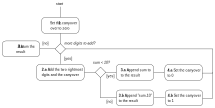
\includegraphics[width=\textwidth]{images/flowchart}
%   \end{center}
%   \caption{A flowchart depicting the addition of two natural numbers}
%   \label{fig:flowchart}
% \end{figure}

% \paragraph{Using Pseudocode} A less space-demanding way is to use some
% pseudo-code\sidenote{I will not use much pseudo code in this
%   course. It is a matter of taste, but I found it very similar to
%   writing high-level languages such as Python or Ruby, which one can
%   run---for free.}. This resemble programming but does not refer to an
% actual language. It just calls for a general understanding of
% programming concepts. Regarding the addition of two numbers, we could
% write something like:

% \begin{algorithm}
%   \KwData{$x,y \in \mathbb{N}^2$}
%   \KwResult{$result = x + y$}
%   $result \gets \emptyset$\;
%   $length \gets \max(length(x), length(y))$\;
%   $index \gets 1$\;
%   $sum \gets 0$\;
%   $carry \gets 0$\;
%   \While{$index \leq length$ or $carry = 1$}{
%     $sum \gets digit(x, index) + digit(y, index) + carry$\;
%     \If{$sum > 9$}{
%       $carry \gets 1$\;n
%       $sum \gets sum - 10$\;
%     }
%     $result \gets append(sum, result)$\;
%     $index \gets index + 1$\;
%   }
% \end{algorithm}

% \paragraph{Using a Program} If we do \emph{not} want to be ambiguous,
% we can directly write a program using your favorite language. I
% put below a Python program equivalent to the pseudo code
% above\sidenote{Writing a program that adds two numbers this way is a
%   complete nonsense. Addition is natively supported in all
%   languages!}.

% \inputminted{python}{code/sum.py}

% \begin{takeaway}
%   An algorithm is a pure abstract concept, which we cannot directly
%   seize. It only surfaces when we describe it using a specific language
%   or syntax.
% \end{takeaway}

% We still have a problem however. When we describe an algorithm, we
% need to decide on \emph{basic actions} and we assume that
% \emph{executor} (either a machine or a human) is able to perform
% these. For example, to add two natural numbers, we have assumed the
% existence of conditional statements, loops, arithmetic and logical
% operations, etc. In the next section, we'll specify these actions using a
% \emph{computation model}, which we will use throughout the remainder
% of this course.

\section{Course Overview}

Are we going to go through a never-ending list of algorithms and
data-structure? In a sense yes, but bear in mind that the point of the
course is to practice solving problems. Algorithms and data
structures are just a means.

\subsection{Syllabus}

Figure~\ref{fig:syllabus} details the topics we will cover. My
strategy is to start with the concepts and theories and then to go
through the data structures and algorithms I think are the most
relevant. The two first weeks focus on the basics: What is an
algorithm, what is a program, how does a computer executes a program,
how to measure time and memory consumption? etc. Then we apply these
again and again on basic algorithms and data structures: Records,
arrays, lists, recursion and sorting.

\begin{figure}[htbp]
  \begin{center}
    \includestandalone[width=.9\textwidth]{images/syllabus.tikz}
  \end{center}
  \caption{Topic covered during the 13 Weeks}
  \label{fig:syllabus}
\end{figure}

Then, we push on to more advanced concepts, including hashing (Week
7), trees (Week 8, 9) and graphs (Week 10). These are all the data
structures we will study but sure there are many more. In the
remainder we will explore two other topics where algorithms play a key
role: Combinatorial search and regular expressions. Finally we will
wrap up with looking at two other computation models: Parallel
computing and Quantum computing. The knowledge we got is very general
and apply there as well.

\begin{takeaway}
  This course is hard: Learning to solve computational problems
  efficiently takes practice.
\end{takeaway}

\paragraph{No Prerequisites} Anyone can join and succeed in this
course: There is no prerequisite. I will use some high-school maths
(functions, sets, probabilities, summations, boolean logic), which I
recall in a separate appendix. The plan is to explain everything we
need as we go. This is \emph{not} a maths class.

\paragraph{Why to Study This?}
As you may already sense, this is the foundations of Computer Science,
and in turn, of Software Engineering. Image processing, cryptography,
compilers, networks, artificial intelligence, and other ``branches''
of Computer Science all develop algorithms and data
structures. Consider image processing as an example: How to detect the
contour of a shape in a bitmap?  What data structure is the most
suitable to represent an image in memory? Which algorithm is the
fastest? Which consume the least memory? This course lay down the
foundations to discuss, evaluate and compare algorithms and data
structures.

Besides, as a software engineer, your daily work is to solve
computation problems! Say we have to sort the score of the top players
in your new mobile game, for instance. Shall we go for a \emph{quick
  sort} or a \emph{radix sort}?  Should we roll out something of our
own? It is critical to know what already exists and where we it shines
and where it falls short.


\subsection{Learning Outcomes}

How will this course contribute to your career? By
developing competencies, skills and knowledge.

\paragraph{Competence}
Again, the point is to develop a single competence: \emph{Solving
  computational problems}, by designing algorithms and programs that a
machine can execute. This is difficult. This is not something we learn
and recite: One must hone this with practice.

\paragraph{Skills}
As we practice solving computational problems, we will build three
core skills:
\begin{enumerate}
\item Design algorithms and data structures tailored for a specific
  problem.
\item Argue for their correctness and be confident that the solution
  we come up with actually solves the problem at hand.
\item Evaluate the time and memory consumed by our algorithms in order
  to compare with alternative solutions.
\end{enumerate}

\paragraph{Knowledge}
This course contains a lot of knowledge, especially in the form of
known problems and their accepted solutions, which combine algorithms
and data structures. This course is not exhaustive at all! It is just
an introduction, but it will give you the shared vocabulary and
culture to be effective as a professional. We will cover the basics:
Arrays, lists, searching, sorting, trees, graphs, hashing, etc.

\begin{takeaway}
  The single objective of this course is to train you at solving
  computational problems. This is hard enough.
\end{takeaway}


\section{Practicalities}
Overall, we have three sessions a week during 13 weeks. Each session is
divided into 30 minutes of lectures and 1h30 of exercises or lab
session.

\paragraph {Lectures}
I broke down the content into 30 minutes long lectures. Each lecture
addresses a specific topic. I use various programming languages as
examples, avoiding those that are too verbose on slides. Keep in mind
that algorithms and data structures apply to any programming
language. I provide written lecture notes for the most important
lectures, so you can focus on understanding.

\paragraph {Lab sessions}
The lab sessions aim at putting concepts into practice. These are
either pen-and-paper exercises or programming tasks. Programming tasks
are in Java, but feel free to use any other language that works better
for you. The point is to solve the programming tasks, not to struggle
with the language. There is however no need to know Java programming
beforehand, but a prior exposure will help. I provide selected written
solution, where I see fit.

\paragraph {Weekly Quizzes}
Every week, I will post a quiz to help you assess your understanding
of the week's topics. They do not account in your grade but please
reach out if any thing is unclear.

\paragraph{Examinations}
Your grade depends solely on the final examination. To get prepared as
well as possible, I include two ``home'' examinations around Week 4 and
8. These are optional, but should you feel the need for it, I can
grade them. All examinations follow the same pattern: 100 points
divided among four parts with 5 questions each.

\section{Expectations}

\paragraph{What do I expect from you?}

\emph{This content is hard}---I cannot stress this enough. Some of
which are non-trivial. Yet, I made everything optional, but the final
examination. I see this course is an opportunity to study algorithms
and data structures. Here is what I \emph{strongly} recommend:

\begin{itemize}
\item Attend the lecture physically. Even more, ask questions!
  Attending empower you to ask questions and to stop me if I am
  unclear. Please do so: I am happy to adjust or answer to the best of
  my knowledge.
\item Attend the lab sessions and go through the exercises. In my
  experience, exercises (whether on paper or on computer) is the only
  thing that really ground our understanding.
\item Go through the home examinations. I believe this is a good
  preparation to the final one and also a good way to see where we
  stand.
\item Reach out if you need any help.
\item Practice. practice, practice.
\end{itemize}

As you can see in Table~\ref{tab:syllabus}, this course is
``content-heavy''. I don't think one can master the whole thing in a
week or so before the final examination. A strongly recommend you
spread your work over the 13 weeks.

\paragraph {What can you expect from me?}

I am there three times a week for all lectures and lab sessions. Feel
free to come and ask questions. Besides these slots, I try to be
available and responsive, by email
especially\sidenote{I am not sitting in NTNU on a daily
  basis. Reaching out by email is the best way to get help.}. I try to
reply within 24 hours, but bear in mind that I am also a full time
engineer. Expect answers outside office hours.


\section{Additional Resources}

There are loads of books
\cite{atto1974,melhorn2008,levitin2011,weiss2014,skiena2020}, videos,
online courses and tutorials on algorithms and data structures. All of
this is basic stuff: I am not presenting anything new or
innovative. Let me know if the angle I have chosen is unclear or does not
fit your taste: We can look at other resources where the same content
is taken from a different perspective.

\emph{I do \textbf{not} follow any textbook} in particular, but there are a few
``references'' textbooks, whose authors are leading authorities in the
field. Feel free to check them if you need a different approach:

\begin{itemize}
\item ``The Art of Computer Programming'' (aka TAOCP) by Donald
  E. Knuth. This is \emph{the} reference. Five volumes so far:
  Fundamentals~\cite{knuth1978}, semi-numerical~\cite{knuth1997},
  sorting and searching~\cite{knuth1998}, combinato\-rial
  al\-go\-ri\-thms~\cite{knuth2011}. I found the treatment very detailed
  and oriented towards the mathematically oriented. Beyond the scope
  of this course.
\item ``Introduction to Algorithms'' by Thomas H. Cormen et
  al~\cite{cormen2009} is another famous reference. It covers most of
  the topic I selected and many more, except maybe random access
  machines.
\item ``Algorithms'' by Robert Sedgewick~\cite{sedgewick2014} is another
  well-known textbook, which is used in some very successful online
  courses. Example are given in Java.
\item ``Data structures and algorithms in Java'' by Michael
  T. Goodrich and Roberto Tamassia~\cite{goodrich2014} fits very well this
  course. Most content we will cover is also treated there.
\end{itemize}

There are also online course on platforms such as
\href{https://www.coursera.org}{Coursera} or
\href{https://www.edx.org}{EdX} for instance. They can be a good
alternative to my presentations. Check however that the content they
cover matches the syllabus.

You will also find many online blog posts and tutorials such as
\href{www.geeksforgeeks.com}{GeeksForGeeks} or
\href{www.tutorialspoint.com}{TutorialsPoint}. Please keep a critical
eye as they may contain mistakes (as does this course).

Finally, there are many web sites such
\href{http://www.hackerrank.com}{HackerRank} or
\href{https://leetcode.com}{LeetCode} where one can practice solving
problems. Many of these problems are direct applications of the
concepts we will study. These web sites are great resources to gain
fluency.


\section*{Conclusions}
Let us get started! There is a lot or ground to cover. Please reach
out if you have any questions or if you find mistakes in the slides,
the lectures notes or the lab sessions.

\bibliographystyle{acm}
\bibliography{references}

\end{document}
